\chapter{RL for {\sc LTL}$_f$/{\sc LDL}$_f$ Goals}

\section{Reinforcement Learning}
\label{RL}
Reinforcement Learning \citep{Sutton:1998:IRL:551283} is a sort of optimization problem where an \emph{agent} interacts with an \emph{environment} and obtains a \emph{reward} for each action he chooses and the new observed state. The task is to maximize a numerical reward signal obtained after each action during the interaction with the environment. The agent does not know a priori how the environment works (i.e. the effects of his actions), but he can make observations in order to know the new state and the reward. Hence, learning is made in a \emph{trial-and-error} fashion. Moreover, it is worth to notice that in many situation reward might not been affected only from the last action but from an indefinite number of previous action. In other words, the reward can be \emph{delayed}, i.e. the agent should be able to foresee the effect of his actions in terms of future expected reward. Figure \ref{fig:agent-environment} represent the interaction between the agent and the environment in this setting.
\begin{figure}[!h]
	\centering
	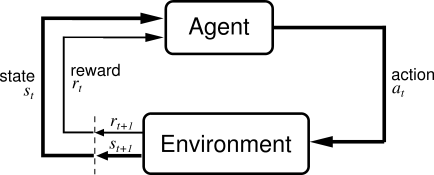
\includegraphics[width=.8\linewidth]{images/agent-environment}
	\caption{The agent and its interaction with the environment in Reinforcement Learning}\label{fig:agent-environment}
\end{figure}

In the next subsections we introduce some of the classical mathematical frameworks for RL: Markov Decision Process (MDP) and Non-Markovian Reward Decision Process (NMRDP).
\section{Markov Decision Process (MDP)}
\label{MDP}

A Markov Decision Process (MDP) $\MDP$ is a tuple $\tup{\States, \Actions, \TrFun, \Reward, \DiscFact}$ containing a set of \emph{states} $\States$, a set of \emph{actions} $\Actions$, a \emph{transition function} $\TrFun: \States \times \Actions \to Prob(\States)$ that returns for every pair state-action a probability distribution over the states, a \emph{reward function} $\Reward: \States \times \Actions \times \States \to \Reals$ that returns the reward received by the agent when he performs action $a$ in $s$ and transitions in $s'$, and a \emph{discount factor} $\DiscFact$, with $0 \le \DiscFact \le 1$, that indicates the present value of future rewards. With $\TrFun(s, a, s')$ we denote the probability to end in state $s'$ given the action $a$ from $s$.

The discount factor $\DiscFact$ deserves some attention. Its value highly influences the MDP, its solution, and how the agent interprets rewards. Indeed, if $\DiscFact = 0$, we are in the pure \emph{greedy} setting, i.e. the agent is shortsighted and look only at the reward that it might obtain in the next step, by doing a single action. The higher $\DiscFact$, the longer the sight horizon, or the foresight, of the agent: the far rewards are taken into account for the  current action choice. If $\DiscFact < 1$ we are in the \emph{finite horizon} setting: namely, the agent is intrinsically motivated to obtain rewards as fast as possible, depending on how $\DiscFact$ is far from $1$. When $\DiscFact = 1$ we are in the \emph{infinite horizon} setting, which means that the agent considers far rewards as they can be obtained in the next step. In other words, we may think the agent as \emph{immortal}, since the time the agent spend to reach rewards does not matter anymore.

\medskip
A \emph{policy} $\Policy: \States \to \Actions$ for an MDP $\MDP$ is a mapping from states to actions, and represents a solution for $\MDP$. Given a sequence of rewards $\Reward_{t+1}, \Reward_{t+2}, \dots, \Reward_{T}$, the \emph{expected return} $\ExpRet_t$ at time step $t$
is defined as: 
\begin{equation}
\ExpRet_t \defeq \sum_{t=k+1}^T \DiscFact^{k-t-1}\Reward_k
\end{equation} where can be $T = \infty$ and $\DiscFact = 1$ (but not both). 

The \emph{value function} of a state $s$, the \emph{state-value function} $\ValFun_\Policy(s)$ is defined as the expected return when starting in $s$ and following policy $\Policy$, i.e.:
\begin{equation}
\label{def:state-value-fun}
\ValFun_\Policy(s) \defeq \mathbb{E}_{\Policy}[\ExpRet_t | \States_t = s], \forall s \in \States
\end{equation}

Similarly, we define $\qFun_\Policy$, the \emph{action-value function for policy $\Policy$}, as:
\begin{equation}
\label{def:action-value-fun}
\qFun_\Policy(s, a) \defeq \mathbb{E}_{\Policy}[\ExpRet_t | \States_t = s, \Actions_t = a], , \forall s \in \States, \forall a \in \Actions
\end{equation}

Notice that we can rewrite \ref{def:state-value-fun} and \ref{def:action-value-fun} recursively, yielding the \emph{Bellman equation}:

\begin{equation}
\label{def:bellman-state-value-fun}
\ValFun_\Policy(s) =  \sum_{s'} P(s' | s,a)[\Reward(s,a,s') + \DiscFact \ValFun(s')] 
\end{equation}

where we used the definition of the transition function:
\begin{equation}
\TrFun(s,a,s') = P(s' | s,a)
\end{equation}

We define the \emph{optimal state-value function} and the \emph{optimal action-value function} as follows:
\begin{equation}
\label{optimal-state-value-fun}
\ValOptFun(s)  \defeq \max_\Policy  \ValFun_\Policy(s), \forall s\in \States		
\end{equation}

\begin{equation}
\label{optimal-action-value-fun}
\qOptFun(s, a) \defeq \max_\Policy  \qFun_\Policy(s, a), \forall s\in \States, \forall a\in \Actions
\end{equation}

Notice that with \ref{optimal-state-value-fun} and \ref{optimal-action-value-fun} we can show the correlation between $\ValOptFun_\Policy(s)$ and $\qOptFun_\Policy(s, a)$:

\begin{equation}
\qOptFun(s, a) = \mathbb{E}_\Policy[R_{t+1} + \DiscFact \ValOptFun_\Policy(\States_{t+1})| \States_t = s, \Actions_t = a]
\end{equation}


We can define a partial order over policies using value functions, i.e. $\forall s\in \States. \Policy \ge \Policy' \iff \ValFun_\Policy(s) \ge \ValFun_{\Policy'}(s)$. 
Now we give the definition of optimal policy:
\begin{definition}\label{def:optimal-policy}
	An \emph{optimal policy} $\OptPolicy$ is a policy such that $\OptPolicy \ge \Policy$ for all $\Policy$. 
\end{definition}

Given an MDP $\MDP$, a typical reinforcement learning problem is the following: find an optimal policy for $\MDP$, without knowing $\TrFun$ and $\Reward$. Notice that instead of explicit specification of the transition probabilities and rewards, the transition probabilities are accessed through a simulator that is restarted many times from a fixed or uniformly random initial state $s_0\in\States$. We call this way of structuring the learning process \emph{episodic reinforcement learning}. Usually, in episodic reinforcement learning, we require the presence of one or more \emph{goal states} where the simulation of the MDP ends and the task is considered completed, or a maximum time limit $T$ for the number of action that can be taken by the agent in one single episode, and the overcoming of $T$ determines the end of the episode. Optionally, \emph{failure states} can be also defined, where the episode end similarly to goal states, but the task is considered failed.

\subsubsection{Examples}
Many dynamic systems can be modeled as Markov Decision Processes. 

\begin{example}[\textbf{Gridworld}] Perhaps the most simple MDP used as a toy example is \emph{Gridworld}, depicted in Figure \ref{fig:gridworld}.
There are $3\times 4$ cells, i.e. states of the MDP $\States = \set{s_{11}, s_{12}, \dots, s_{34}}\setminus \set{s_{22}}$. The agent can do four actions: $A = \set{Right, Left, Up, Down}$. The initial state is fixed and is $s_0 = s_{11}$ and the agent can move in any of the adjacent and free cells from the current state. Assuming an episodic task, the goal is to reach $s_{34}$, and $s_{24}$ represent a failure state. The state transition function $\TrFun$ can be \emph{deterministic}, i.e. the agent always succeed in performing actions, or non-deterministic, i.e. the effect of an action is determined by the probabilistic distribution returned by $\TrFun(s, a)$. An example of non-deterministic $\TrFun$ is to give $90\%$ of success (the agent moves in the chosen direction) and $10\%$ of fail (the agent moves at either the right or left angle to the intended direction). If the move would make the agent walk into a wall (borders of the grid and $s_{22}$), the agent stays in the same place as before. The reward function $R(s,a,s')$ is defined as $-1$ if $s'=s_{24}$, as $1$ if $s'=s_{34}$, and $-0.01$ otherwise. The small negative reward given at each transition is a popular mean for reward function design: it is called \emph{step reward} and its purpose is to encourage the agent to finish the episode as fast as possible, with a priority proportional to the absolute value of the reward. The discount factor $\DiscFact$ should be strictly higher than 0 because more than one step is needed to reach the goal state.
	
\begin{figure}[h]
	\centering
	\caption{The Gridworld environment}\label{fig:gridworld}
	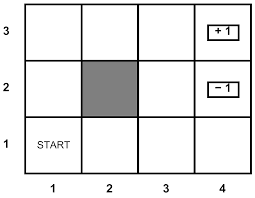
\includegraphics[width=.4\linewidth]{images/gridworld}
\end{figure}

An example of optimal policy is shown in Figure \ref{gridworld-optimal-policy}. As the reader can notice, the arrows represent the action that should be taken in a certain cell, in order to maximize the expected return. We observe that the optimal action in $s_{13}$, according to the policy, is not the one to take the shortest path to the goal, i.e. the $Up$ action. This is because there is a small probability to ends in $s_{24}$, the failure state, and be punished with a high negative reward. In terms of expected reward, it is better to take the longer path, at the price of collect small negative rewards, but avoiding the risk to fail miserably.
\begin{figure}
	\centering
	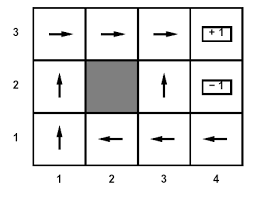
\includegraphics[width=.4\linewidth]{images/gridworld-optimal-policy}
	\caption{An example of optimal policy for the Gridworld environment}\label{gridworld-optimal-policy}. 
\end{figure}

\end{example}

\begin{example}[\textbf{Breakout}]
	\begin{figure}
		\centering
		
\includegraphics[width=.6\linewidth]{images/breakout.jpg}
		\caption{A screenshot from the videogame \Breakout}\label{breakout}. 
	\end{figure}
\end{example}

\section{Temporal Difference Learning}
\label{sect:temporal-difference-learning}
\emph{Temporal difference learning} (TD) \citep{Sutton1988} refers to a class of model-free reinforcement learning methods which learn by bootstrapping from the current estimate of the value function. These methods sample from the environment, like Monte Carlo (MC) methods, and perform updates based on current estimates, like dynamic programming methods (DP) \citep{Bellman:1957}. We do not discuss MC and DP methods here.

Q-Learning \citep{watkins1989learning, Watkins1992} and SARSA are such a methods. They update $\qFunEst(s, a)$, i.e. the estimation of $\qOptFun(s, a)$ at each transition $(s, a) \to (s', r)$. The update rule is the following:
\begin{equation}\label{td-update-rule}
\qFunEst(s, a) \leftarrow \qFunEst(s, a) + \LRate \delta
\end{equation}
where $\delta$ is the \emph{temporal difference}. In SARSA, it is defined as:
\begin{equation}
\delta = r + \DiscFact \qFunEst(s', a') - \qFunEst(s, a)
\end{equation}
whereas in Q-Learning:
\begin{equation}
\delta = r + \DiscFact \max_{a'} \qFunEst(s', a') - \qFunEst(s, a)
\end{equation}

TD$(\lambda)$ is an algorithm which uses \emph{eligibility traces}. The parameter $\lambda$ refers to the use of an eligibility trace. The algorithm generalizes MC methods and TD learning, obtained respectively by setting $\lambda = 1$ and $\lambda = 0$. Intermediate values of $\lambda$ yield methods that are often better of the extreme methods. 
Q-Learning and SARSA that has been shown before can be rephrased with this new formalism as Q-Learning(0) and SARSA(0), special cases of Watkin's Q$(\lambda)$ and SARSA($\lambda$) respectively.
In this setting, Equation \ref{td-update-rule} is modified as follows:
\begin{equation}\label{td-lambda-update-rule}
\qFunEst(s, a) \leftarrow \qFunEst(s, a) + \LRate \delta e(s, a)
\end{equation}

Where $e(s, a) \in [0, 1]$, the \emph{eligibility of the pair $(s, a)$}, determines how much the temporal difference $\delta$ should be weighted.
SARSA($\lambda$) is reported in Algorithm \ref{alg:sarsa-lambda}, whereas Watkin's Q($\lambda$) in Algorithm \ref{alg:q-learning-lambda}, both  in the variants using \emph{replacing eligibility traces} (see line \ref{sarsa-lambda-replacing-traces} and line \ref{q-learning-lambda-replacing-traces}, respectively).
\begin{algorithm}
	\caption{SARSA($\lambda$) \citep{Singh:1996:RLR:225667.225679}}
	\label{alg:sarsa-lambda}
	\begin{algorithmic}[1]
		\State Initialize $Q(s, a)$ arbitrarily and $e(s, a)=0$ for all $s, a$
		
		\Repeat \{for each episode\} 
			\State initialize $s$
			\State Choose $a$ from $s$ using policy derived from $Q$ (e.g. $e$-greedy)
			\Repeat \{for each step of episode\}
				\State Take action $a$, observe reward $r$ and new state $s'$
				\State Choose $a'$ from $s'$ using policy derived from $Q$
				\State $\delta \gets r + \gamma Q(s', a') - Q(s, a)$
				\State $e(s, a) \gets 1$ \Comment{replacing traces} \label{sarsa-lambda-replacing-traces}
				\For{$\mathbf{all}\ s, a$}
					\State $Q(s, a) \gets Q(s, a) + \alpha\delta e(s, a)$
					\State $e(s, a) \gets \DiscFact\lambda e(s, a)$
				\EndFor
				\State $s\gets s'$, $a \gets a'$
			\Until state $s$ is terminal
		\Until
	\end{algorithmic}
	
\end{algorithm}
\begin{algorithm}
	\caption{Watkin's Q($\lambda$) \citep{watkins1989learning}}
	\label{alg:q-learning-lambda}
	\begin{algorithmic}[1]
		\State Initialize $Q(s, a)$ arbitrarily and $e(s, a)=0$ for all $s, a$
		\Repeat \{for each episode\} 
			\State initialize $s$
			\State Choose $a$ from $s$ using  policy derived from $Q$ (e.g. $e$-greedy)
			\Repeat \{for each step of episode\}	
				\State Take action $a$, observe reward $r$ and new state $s'$
				\State Choose $a'$ from $s'$ using policy derived from $Q$ (e.g. $e$-greedy)
				\State $a^* \gets \arg\max_a Q(s', a)$ (if $a'$ ties for max, then $a^* \gets a'$)
				
				\State $\delta \gets r + \gamma Q(s', a^*) - Q(s, a)$
				\State $e(s, a) \gets 1$ \Comment{replacing traces}\label{q-learning-lambda-replacing-traces}
				\For{$\mathbf{all}\ s, a$}
					\State $Q(s, a) \gets Q(s, a) + \alpha\delta e(s, a)$
					\If{$a' = a^*$}
						\State $e(s, a) \gets \DiscFact\lambda e(s, a)$
					\Else 
						\State $e(s, a) \gets 0$
					\EndIf
					
					\State $e(s, a) \gets \DiscFact\lambda e(s, a)$
				\EndFor
				\State $s\gets s'$, $a \gets a'$
			\Until state $s$ is terminal
		\Until
	\end{algorithmic}
	
\end{algorithm}

\section{Non-Markovian Reward Decision Process (NMRDP)}\label{sect:NMRDP}
For some goals, it might be the case that the Markovian assumption of the reward function $\Reward$ -- that reward depends only on the current state, and not on history -- does not hold. Indeed, for many problems, it is not effective that the reward is limited to depend only on a single transition $(s,a,s')$; instead, it might be extended to depend on \emph{trajectories} (i.e. $\traj$), e.g. when we want to reward the agent for some (temporally  extended) behaviors, opposed to simply reaching certain states. 

This idea of rewarding behaviors has been proposed by \citep{bacchus1996rewarding} where they defined a new mathematical model, namely Non-Markovian Reward Decision Process (NMRDP), and showed how to construct optimal policies in this case.

In the next subsections, we give the main definitions to reason in this new setting. Then we show the solution proposed in \citep{bacchus1996rewarding}.

\subsection{Preliminaries}
Now follows the definition of NMRDP, which is similiar to the MDP definition given in Section \ref{MDP}.

\begin{definition}\label{def:nmrdp}
	A Non-Markovian Reward Decision Process (NMRDP) \citep{bacchus1996rewarding} $\NMRDP$ is a tuple $\tup{\States, \Actions, \TrFun, \NMReward, \DiscFact}$ where $\States, \Actions, \TrFun$ and $\DiscFact$ are defined as in the MDP, and $\NMReward : \States^* \to \Reals$ is the \emph{non-Markovian reward function}, where $\States^* = \set{\projtraj_{n\ge0, s_i\in\States}}$ is the set of all the possible traces, i.e. projection of trajectories $\traj$
	
\end{definition}

Given a trace $\trace = \projtraj$, the \emph{value of $\trace$} is:
\begin{equation}
v(\pi) = \sum_{i=1}^{|\trace|} \DiscFact^{i-1}\NMReward(\projtraj)
\end{equation}
where $|\trace|$ denotes the number of transitions (i.e. of actions).

The policy $\NMPolicy$ in this setting is defined over sequences of states, i.e. $\NMPolicy: \States^* \to \Actions$. The \emph{value of $\NMPolicy$} given an initial state $s_0$ is defined as:

\begin{equation}
\ValFun^{\NMPolicy}(s) = \mathbb{E}_{\pi \sim \NMRDP, \NMPolicy, s_0}[v(\pi)]
\end{equation}

i.e. the expected value in state $s$ considering the distribution of traces defined by the transition function of $\NMRDP$, the policy $\NMPolicy$ and the initial state $s_0$.

We are interested in two problems, that we will study in the next sections:
\begin{itemize}
	\item Find an optimal (non-Markovian) policy $\NMPolicy$ for an NMRDP $\NMRDP$ (Definition \ref{def:nmrdp});
	\item Define the non-Markovian reward function for the domain of interest.
\end{itemize}

\subsection{Find an optimal policy $\NMPolicy$ for NMRDPs}\label{nmrdp-find-optimal-policy}
The  key  difficulty  with  non-Markovian  rewards  is  that
standard optimization techniques, most based on Bellman's \citep{Bellman:1957} 
dynamic  programming  principle,  cannot  be  used. Indeed, this requires one 
to resort to optimization over a policy space that maps histories
(rather than states)  into actions, a process that would incur great 
computational expense. \citep{bacchus1996rewarding} give the definition of 
a decision  problem \emph{equivalent} to an NMRDP  in  which  the  rewards  are
Markovian. This construction is the key element to solve our problem,
i.e. find an optimal policy for an NMRDP.


\subsubsection{Equivalent MDP}
Now we give the definition of \emph{equivalent} MDP of an NMRDP, and state an important result. 

\begin{definition}[\cite{bacchus1996rewarding}]
	\label{nmrdp-mdp-equivalence}
	An NMRDP $\NMRDP = \tup{\States, \Actions, \TrFun, \NMReward, \DiscFact}$ is \emph{equivalent} to an extended
	MDP $\MDP = \tup{\States', \Actions, \TrFun', \Reward', \DiscFact}$ if there exist two functions 
	$\tau: \States' \to \States$ and $\sigma: \States\to \States'$ such that
	\begin{enumerate}
		\item $\forall s \in \States: \tau (\sigma(s)) = s$; \label{nmrdp-mdp-equivalence-cond1}
		\item $\forall s_1, s_2 \in \States$ and $s_1' \in \States'$: if $\TrFun(s_1 , a, s_2 ) > 0$ and $\tau (s'_1) =
		s_1$, there exists a unique $s'_2 \in \States'$ such that $\tau (s'_2 ) = s_2$ and
		$\TrFun'(s'_1 , a, s'_2 ) = \TrFun(s_1, a, s_2 )$;
		\label{nmrdp-mdp-equivalence-cond2}
		\item For any feasible trace $\projtraj$ of $\NMRDP$
		and $\projtrajprime$ of $\MDP$ associated to the trajectories $\traj$ and $\trajprime$, such that $\tau(s'_i) = s_i$
		and $\sigma(s_0) = s'_0$, we have $R(\projtraj) =
		R'(s_{n-1}, a_{n-1}, s'_n)$.
		\label{nmrdp-mdp-equivalence-cond3}	
	\end{enumerate}
\end{definition}

Given the Definition \ref{nmrdp-mdp-equivalence}, we give the definition of corresponding policy:
\begin{definition}[\cite{bacchus1996rewarding}]\label{nmrdp-mdp-policy-equivalence}
	Let $\NMRDP$ be an NMRDP and let $\MDP$ be the equivalent MDP as defined in Definition \ref{nmrdp-mdp-equivalence}.
	Let $\Policy$ be  a  policy  for $\MDP$. The 
	\emph{corresponding policy} for $\NMRDP$ is  defined  as 
	$\NMPolicy(\tup{s_0, \dots, s_n}) = \Policy(s'_n) $,   where for the sequence $\tup{s'_0, \dots, s'_n}$ we have $\tau(s'_i) = s_i\ \forall i$ and $\sigma(s_0)=s'_0$
\end{definition}
From definitions \ref{nmrdp-mdp-equivalence} and 
\ref{nmrdp-mdp-policy-equivalence}, and since that for all 
policy $\Policy$ of $\MDP$ the corresponding policy 
$\NMPolicy$ of $\NMRDP$ is such that $ \forall s. \ValFun_\Policy(s) = \ValFun_{\NMPolicy}(\sigma(s))$, the following theorem holds:
\begin{theorem}[\cite{bacchus1996rewarding}]\label{nmrdp-mdp-equivalence-policy-optimality}
	Let $\Policy$ be an  optimal policy for MDP $\MDP$. Then the corresponding policy is optimal for NMRDP $\NMRDP$.
\end{theorem}

The Theorem \ref{nmrdp-mdp-equivalence-policy-optimality} allow us to learn an optimal policy $\NMPolicy$ for NMRDP by learning a policy $\Policy$ over an equivalent MDP, which can be done by resorting on  any off-the-shelf algorithm (e.g. see Section \ref{sect:temporal-difference-learning}). Moreover, obtaining the corresponding policy for the original NMRDP is straightforward, although in practice is not needed, since it is enough to run the policy $\Policy$ over the MDP.

In other words, the problem of finding an optimal policy for an NMRDP reduces to find an optimal policy for an equivalent MDP such that Condition 1, 2 and 3 of Definition \ref{nmrdp-mdp-equivalence} hold.


\subsection{Define the non-Markovian reward function $\NMReward$}
To  reward  agents  for  (temporally  extended)
behaviors, as opposed to simply reaching certain states, we need a way
to specify rewards for specific trajectories through the state
space. 
Specifying a non-Markovian reward function explicitly is quite hard and unintuitive, impossible if we are in a infinite-horizon setting. 
Instead, we can define \emph{properties} over trajectories and reward only the ones which satisfy some of them, in contrast to enumerate all the possible trajectories.

Temporal logics presented in Section \ref{sect:ltl} gives an effective way to do this. 
Indeed, in order to speak about a desired behavior,  i.e. fulfillment of properties that might change over time, we can define a \emph{formula} $\varphi$ (or more formulas) in some suited temporal logic formalism semantically defined over trajectories $\trace$, speaking about a set of properties $\Prop$ such that each state $s\in S$ is associated to a set of propositions ($S\subseteq 2^\Prop$). 
In this way, a trajectory $\trace = \traj$ is rewarded with $r_i$ iff $\trace \models \varphi_i$, where $r_i$ is the reward value associated to the fulfillment of behaviors signified by $\varphi_i$.

\subsection{Using \PLTL}
\label{sect:using-pltl}
In \citep{bacchus1996rewarding} the temporal logic formalism is \emph{Past Linear Temporal Logic} (\PLTL), which is a past version of \LTL (Section \ref{sect:ltl}).
As explained before, using the declarativeness of \PLTL, is possible to specify the desired behavior (expressed in terms of the properties $\Prop$) that should be satisfied by the experienced trajectories and reward only them, hence obtaining a non-Markovian reward function. More formally, given a finite set $\Phi$ of \PLTL \emph{reward formulas}, and for each $\phi_i \in \Phi$ a real-valued reward $r_i$, the \emph{temporally extended reward function} $\bar{R}$ is defined as:
\begin{equation}\label{pltl-temp-extended-reward-fun}
\NMReward(\projtraj) = \sum_{\phi_i \in \Phi : \tup{s_0, s_1, \dots, s_n}\models \phi_i} r_i
\end{equation}


In order to run the actual learning task, \citep{bacchus1996rewarding} proposed a transformation from the NMRDP to an equivalent MDP with the state space \emph{expaneded} which allows to label each state $s\in \States$. The idea is that the labels should 
keep track in some way the (partial) satisfaction of the temporal formulas $\phi_i \in \Phi$. 
A state $s$ in the transformed state space is replicated multiple times, marking the difference between different (relevant) histories terminating in state $s$.

In this way, they obtained a compact representation of the required history-dependent policy
by considering only relevant history, and can produce this
policy using computationally-effective MDP algorithms.
In other words, the states of the NMRDP can be mapped into those of the expanded MDP, 
in such a way that corresponding states yield
same transition probabilities and corresponding traces have same rewards.

\section{NMRDP with \LTLf/\LDLf rewards}\label{sect:nmrdp-llf-rewards}
In this section we explain how to specify non-Markovian rewards with \LTLf/\LDLf  formulas (instead of \PLTL) and how the associated MDP expansion works \citep{Brafman2017SpecifyingNR}, analogously to what we saw with \PLTL (Section \ref{sect:using-pltl}).

The temporally extended reward function $\bar{R}$ is similar to Equation \ref{pltl-temp-extended-reward-fun}, but instead of using \PLTL formula we use \LLf formulas. Formally, given a set of pairs $\set{(\varphi_i, r_i)^m_{i=1}}$ (where $\varphi_i$ denotes the \LLf formula for specifying a desired behavior, and $r_i$ denotes the reward associated to the satisfaction of $\varphi_i$, and given a (partial) trace $\trace = \projtraj$, we define $\bar{R}$ as:
\begin{equation}
\NMReward(\trace) = \sum_{1\le i\le m: \trace \models \varphi_i} r_i
\end{equation}
For the sake of clarity, in the following we use $\set{(\varphi_i, r_i)^m_{i=1}}$ to denote $\bar{R}$.

Now we describe the MDP expansion for doing learning in this setting, as proposed in \citep{Brafman2017SpecifyingNR}. 
Without loss of generality, we assume that every NMRDP $\NMRDP$ is reduced into another NMRDP $\NMRDP'=\tup{\States', \Actions', \TrFun', \Reward', \DiscFact}$:


\begin{gather}
	\begin{split}
	\States' &= \States\cup \set{s_{init}}\\
	\Actions' &= \Actions\cup \set{start}\\
	\TrFun'(s,a,s')  &=  \begin{cases}
			1 & \tm{if\ } s=s_{init}, a=start, s'=s_0\\
			0 & \tm{if\ } s=s_{init} \tm{and} (a\neq start \tm{or} s'\neq s_0)\\
			\TrFun(s, a, s') &  \tm{otherwise}\\
		\end{cases}\\
	\Reward'(\tup{s_{init}, s_0, \dots, s_n}) &= \Reward(\projtraj)
	\end{split}
	\label{nmrdp-adapted}
\end{gather}



and $s_{init}$ is the new initial state. In other words, we prefix to every feasible trajectory $\NMRDP$ the pair $\tup{s_{init}, start}$, denoting the beginning of the episode. 
We do this for two reasons: allow to evaluate formulas in $s_0$ and make it compliant with the most general definition of the reward, namely $R(s, a, s')$, also when there is no true action that is done (i.e. empty trace).

\begin{definition}[\cite{Brafman2017SpecifyingNR}]\label{nmrdp-mdp-transformation-brafman}
	Given an NMRDP $\NMRDP = \tup{S, A, \TrFun, \set{(\varphi_i, r_i)^m_{i=1}, \DiscFact}}$ (i.e. with non-Markovian rewards specified by \LLf formulas) it is possible to build an  $\MDP = \tup{\States', \Actions, \TrFun', \Reward', \DiscFact}$ that is \emph{equivalent} (in the sense of Definition \ref{nmrdp-mdp-equivalence}) to $\NMRDP$. Denoting with 
	$\automaton_{\varphi_i} = \tup{2^\P, Q_i, q_{i0}, \delta_i,F_i}$ (notice that $S\subseteq 2^{\Prop}$ and $\delta_i$ is total) the \DFA associated 
	with $\varphi_i$ (see Section \ref{sect:llf2automata}), the equivalent MDP $\MDP$ is built as follows:
	\begin{itemize}
		\itemsep=0mm
		\item $S'=Q_1\times\cdots\times Q_m\times \States$ is the set of states;
		\item $\TrFun' : S'\times A \times S'\rightarrow [0,1]$ is defined as follows:
		\[
		\begin{array}{l}
		\Tr'(q_1,\ldots,q_m, s, a, q'_1,\ldots,q'_m, s') = {}\\
		\quad\left\{
		\begin{array}{ll}
			Tr(s,a,s') &\mbox{if } \forall i:\delta_i(q_i,s') = q'_i\\
			0 & \mbox{otherwise}; 
			\end{array}\right.
		\end{array}
		\] 
		\item $R': S'\times A \times S'\rightarrow 
		\mathbb{R}$ is defined as:
		\[
		R'(q_1,\ldots,q_m, s, a, q'_1,\ldots,q'_m, s') = 
		%\sum_i \{\rew(\Phi_i) \mid \delta(q_i,t) \in F_i\} 
		\sum_{i: q_i'\in F_i} r_i
		\] 
	\end{itemize}
\end{definition}


\begin{theorem}[\cite{Brafman2017SpecifyingNR}]\label{th:nmrdp-mdp-llf-equivalence}
	The NMRDP $\NMRDP= \tup{\States, \Actions, \TrFun, \{(\varphi_i,r_i)\}_{i=1}^{m}, \DiscFact}$ is equivalent to the  MDP $\MDP= \tup{\States',\Actions,\TrFun',\Reward', \DiscFact}$ defined in Definition \ref{nmrdp-mdp-transformation-brafman}.
\end{theorem}
\begin{proof}
	Recall that every $s' \in S'$ has the form $(q_1 ,\dots, q_m , s)$.
	Define $\tau(q_1 ,\dots, q_m, s) = s$. Define $\sigma(s) = (q_{10} ,\dots, q_{m0}, s)$.
	We have $\tau(\sigma(s)) = s$, hence Condition \ref{nmrdp-mdp-equivalence-cond1} is verified. Condition \ref{nmrdp-mdp-equivalence-cond2} of Definition \ref{nmrdp-mdp-equivalence} is easily verifiable by inspection. For Condition \ref{nmrdp-mdp-equivalence-cond3}, consider a possible trace
	$\trace = \projtraj$. We use $\sigma$ to obtain $s'_0 = \sigma(s_0)$
	and given $s_i$, we define $s'_i$ (for $1 \le i \le n$) to be the unique
	state $(q_{1,i} ,\dots, q_{m,i} , s_i)$ such that $q_{j,i} = \delta(q_{j,i-1}, s_i )$ for all
	$1 \le j \le m$. Moreover, we require that, without loss of generality, every trajectory in the new MDP starts from $s_{init}$ and  now have a corresponding possible trace of
	$\MDP$ , i.e., $\trace = \projtrajprime$. This is the only feasible trajectory of $\MDP$ that satisfies Condition \ref{nmrdp-mdp-equivalence-cond3}. The reward at
	$\trace = \projtraj$ depends only on whether or not
	each formula $\varphi_i$ is satisfied by $\trace$. However, by construction
	of the automaton $\automaton_{\varphi_i}$ and the transition function $\TrFun$, $\trace \models \varphi_i$
	iff $s'_{n} = (q_1 ,\dots, q_m, s_n)$ and $q_i \in F_i$
\end{proof}


Let $\Policy'$ be a (Markovian) policy for $\MDP$. It is easy to define an \emph{corresponding} policy on $\NMRDP$, i.e., a policy that guarantees the same rewards, by using $\tau$ and $\sigma$ mappings defined in Theorem \ref{th:nmrdp-mdp-llf-equivalence} and the result shown in Theorem \ref{nmrdp-mdp-policy-equivalence}.

Obviously, typical learning techniques, such as Q-learning
or SARSA,  are applicable on the expanded
$\MDP$ and
so we can learn an optimal policy $\Policy$ for $\MDP$. 
%%
Thus, an optimal policy for $\NMRDP$ can be learnt on $\MDP$. 
Of course, none of these structures is (completely) 
known to the learning agent, and the above transformation is 
never done explicitly. Rather, the agent carries out the learning process
by assuming that the underlying model is $\MDP$ instead of $\NMRDP$ (applying the fix introduced in Definition \ref{nmrdp-adapted}).


Observe that the state space of $\MDP'$ is the product of 
the state spaces of $\NMRDP$ and $\automaton_{\varphi_i}$, and that the reward
$\Reward'$ is Markovian. In other words, the (stateful) structure of
the \LLf formulas $\varphi_i$ used in the 
(non-Markovian) reward of $\NMRDP$ is \emph{compiled} into 
the states of $\MDP$.

\subsection*{Why should we use \LDLf}
\LDLf formalism (introduced in Section \ref{sect:ldlf})  has the advantage of \emph{enhanced expressive power} over other proposals, as discussed in \citep{Brafman2017SpecifyingNR}. Indeed, we move from linear-time temporal logics to \LDLf, paying no additional (worst-case) complexity costs. \LDLf can encode in polynomial time \LTLf, regular expressions (\REGEX) and the past \LTL (\PLTL) of \citep{bacchus1996rewarding}.
%	, and all examples of (Thiébaux et al. 2006). 
	Moreover, \LDLf can naturally
	represent "procedural constraints" \citep{Baier:2008:BCP:1620270.1620321}, i.e.,
	sequencing constraints expressed as programs, using "if" and
	"while", hence allowing to express more complex properties.


\section{RL for \LTLf/\LDLf Goals}

In this section we define a particular problem and propose a solution, which is the main theoretical contribution of this work. We call this problem \emph{Reinforcement Learning for \LLf Goals}. 

\subsection{Problem definition}

\subsubsection{the World, the Agent and the Fluents}
Let $\W$ be a \emph{world} of interest (e.g. a room, an environment, a videogame). Let $W$ be the set of \emph{world states}, i.e. the states of the world $\W$. 
A \emph{feature} is a function $f_j$ that maps a world state to the
values of another domain $D_j$, such as reals, finite enumerations,
booleans, etc., i.e., $f_j : W \rightarrow D_j$.
%%
Given a set of features $F = \tup{f_1, \dots, f_d}$, the \emph{feature vector} of a world state $w_h$ is the vector
$\mathbf{f}(w_h) = \langle f_1(w_h), \ldots, f_d(w_h) \rangle$ of
feature values corresponding to $w_h$.
%%

Now consider an agent that lives in $\W$. The agent can interact with $\W$ by executing an action $a$ taken from a \emph{set of actions} $\Actions$. Without loss of generality, we assume that such learning agent has a special action $\Stop$ which deems the end of an episode.
Moreover, the agent has its own set of features $F_{ag} = \tup{f_1, \dots, f_d}$, which yields its \emph{representation of the world} $\States$, where $\States \subseteq F_{ag}(W)$ and $F_{ag}(W) = \set{\mathbf{f}_{ag}(w) | w \in W}$. Finally, assume that the agent has a \emph{clock} which determines the granularity of its acting. At every clock, the agent can do action $a$ and observe the new state $s$ from the new world state $w'$, namely $s = \mathbf{f}_{ag}(w)$.

We consider arbitrary \LLf formulas $\varphi_i$
($i=1,\ldots,m$) over a set of fluents $\F$ used for provide a high-level description of the world. We denote by $\L=2^\F$ the set of possible fluents configurations. 
Given a set of feature $F_{goal}$, a \emph{configuration of fluents} $\ell_h \in \L$ is formed by the components that assign truth values to the fluents according to
the feature vector $\mathbf{f}_{goal}(w_h)$. At every step, the features for fluents evaluations are observed, obtaining a particular configuration $\ell\in\L$. Notice that in general the features for the fluents and for the agent state space may differ. The formula $\varphi_i$ is
selecting sequences of fluents configurations $\ell_1,\cdots,\ell_n$,
with $\ell_k\in \L$, whose relationship with the sequences of states
$s_1,\ldots, s_n$, with $s_k \in S$ is unknown.

 In other words, a subset of features are used to describe agent states $s_h$ and another  subset (for simplicity, assumed disjoint from the previous one) are used to evaluate the fluents in $\ell_h$.
 %%
 Hence, given a sequence $w_1,\ldots,w_n$ of
 world states we get the corresponding sequence of sequences learning
 agent states $s_1,\ldots,s_n$ and simultaneously the sequence of fluent
 configurations $\ell_1,\ldots,\ell_n$.  Notice that we do not have a
 formalization for $w_1,\ldots,w_n$ but we do have that for $s_1,\ldots,s_n$
 and for $\ell_1,\ldots,\ell_n$. 


%\begin{itemize}
%	\item We consider a learning agent constituted by MDP
%	$\MDPagent = \tup{\States, \Actions, \TrFun, \Reward, \DiscFact}$ with transition $\TrFun$  and $\Reward$ unknown and
%	sampled from the environment. The true states of the world are observed and mapped into features that compose the state space $\States$ of the agent, or the agent's \emph{representation of the world}, which is the one used for learning.
%	%(e.g., a learning agent for Breakout).  
%	Without loss of generality, we assume that such learning agent has a special action $\Stop$ which
%	deems the end of an episode.
%	
%	\item We consider arbitrary \LLf formulas $\varphi_i$
%	($i=1,\ldots,m$) over a set of fluents $\F$ used for provide a high-level description of the world. We denote by $\L=2^\F$ the set of possible fluents configurations. At every step, the features for fluents evaluations are observed, obtaining a particular configuration $\ell\in\L$. Notice that in general the features for the fluents and for the agent state space may differ. The formula $\varphi_i$ is
%	selecting sequences of fluents configurations $\ell_1,\cdots,\ell_n$,
%	with $\ell_k\in \L$, whose relationship with the sequences of states
%	$s_1,\ldots, s_n$, with $s_k \in S$ of $\MDPagent$ is unknown.
%	
%	\item We are interested in devising a policy for the learning agent
%	$\MDPagent$ such that at the end of the episode, i.e., when the agent
%	executes \emph{stop}\footnote{Note that the agent is unaware that
%		\emph{stop} ends the episode.}, the \LTLf /\LDLf goal formulas
%	$\varphi_i$ ($i=1,\ldots,m$) are satisfied. More precisely, given
%	rewards $r_i$ to be assigned to (complete) episodes satisfying
%	formula $\varphi_i$ ($i=1,\ldots,m$), we want to learn a
%	(non-Markovian) policy
%	%of the form \[\Policy:S^*\rightarrow A\] 
%	that is optimal wrt the sum of the rewards $r_i$
%	($i=1,\ldots,m$) and $R$ in $\MDPagent$. 
%\end{itemize}

Oversimplifying, we may say that $S$ is the set of configurations of
the low-level features for the learning agent, while $\L$ is
the set of configuration of the high-level features needed for
expressing $\varphi_i$.

%Note that both are features in the sense that they are a
%representation of properties of the world but they look at different
%facets of the world itself.
%
%%%
%More precisely, let $W$ be the set of \emph{world states}, i.e., the
%states of the real world.
%%%
%A \emph{feature} is a function $f_j$ that maps a world state to the
%values of another domain $D_j$, such as reals, finite enumerations,
%booleans, etc., i.e., $f_j : W \rightarrow D_j$.
%%%
%The \emph{feature vector} of a world state $w_h$ is the vector
%$\mathbf{f}(w_h) = \langle f_1(w_h), \ldots, f_d(w_h) \rangle$ of
%feature values corresponding to $w_h$.
%%%
%Given a state of the world $w_h$ the corresponding \emph{configuration
%	$s_h$ of the learning agent $\MDPagent$} is formed by the components of
%the feature vector $\mathbf{f}(w_h)$ that produce its state, while the
%corresponding \emph{configuration of fluents} $\ell_h$ is formed by
%the components that assign truth values to the fluents according to
%the feature vector $\mathbf{f}(w_h)$.
%%%
%In other words, a subset of features are used to describe agent states $s_h$ and another  subset (for simplicity, assumed disjoint from the previous one) are used to evaluate the fluents in $\ell_h$.
%%%
%Hence, given a sequence $w_1,\ldots,w_n$ of
%world states we get the corresponding sequence of sequences learning
%agent states $s_1,\ldots,s_n$ and simultaneously the sequence of fluent
%configurations $\ell_1,\ldots,\ell_n$.  Notice that we do not have a
%formalization for $w_1,\ldots,w_n$ but we do have that for $s_1,\ldots,s_n$
%and for $\ell_1,\ldots,\ell_n$. 
\subsubsection{Markovian assumption of the state transition function}
Now we make the following assumption: that is, the agent actions in $A$ induce a transition distribution over the features and
fluents configuration, i.e.,
\begin{equation}\label{joint-tr-fun}
\TrFun_{ag}^{g} : S\times \L \times A \rightarrow Prob(S\times \L)
\end{equation}
This means that the state transition function $\TrFunAgentGoal$ is \emph{Markovian}, i.e. the probability to end in the next state $s'$ with the next fluents configuration $\ell'$ depends only from $s, \ell$ and $a$ (the current agent state, the current fluents configuration and the action taken, respectively).

%Such a transition distribution together with the initial values of the
%fluents $\ell_0$ and of the agent state $s_0$ allow us to describe a
%probabilistic transition system accounting for the dynamics of the
%fluents and agent states.  Moreover, when $\TrFun_{ag}^{g}$ is projected on
%$S$ only, i.e., the $\L$ components are marginalized, we get $\TrFun$ of
%$\MDPagent$. Obviously, both $\TrFun_{ag}^{g}$ and $\TrFun$ are unknown to the learning agent. 
%On the other hand, in response to an agent action $a_h$ performed in the current state
%$w_h$ (in the state $s_h$ of the agent and the
%configuration $\ell_h$ of the fluents), the world changes into $w_{h+1}$ from which $s_{h+1} $ and $\ell_{h+1}$. This is all we need to proceed.

Such a transition distribution together with the initial values of the
fluents $\ell_0$ and of the agent state $s_0$ allow us to describe a
probabilistic transition system accounting for the dynamics of the
fluents and agent states. 
In other words, in response to an agent action $a_h$ performed in the current state
$w_h$ (in the state $s_h$ of the agent and the
configuration $\ell_h$ of the fluents), the world changes into $w_{h+1}$ from which $s_{h+1} $ and $\ell_{h+1}$. This is all we need to proceed.

Notice that we do not assume nothing about the primitive state transitions function, i.e. the one induced over the agent state space $\States$ and the one over the set of possible fluents configurations $\L$. However, it might be the case that the Markovian assumption of the agent state transition function holds, i.e. the probability distribution for the next state $s'$ is fully determined by the current state $s$ and the action $a$. In that case, the considerations presented in this section still holds, since it is a special case of our general assumptions. We only require that the \emph{joint} transition function in Equation \ref{joint-tr-fun} satisfies the Markov property.

\medskip
We are interested in devising policies for the learning agent such that
at the end of the episode, i.e., when the agent executes \emph{stop},
the \LTLf /\LDLf goal formulas $\varphi_i$ ($i=1,\ldots,m$)  are satisfied.
%%
Now we can state our problem formally.

\noindent
\textbf{Problem definition:} \textit{
	We define \emph{RL for \LTLf /\LDLf goals}, denoted as
	\[\MDPagent^{goal}= \tup{\States, \Actions, \Reward, \L, \TrFunAgentGoal, \{(\varphi_i,r_i)\}_{i=1}^{m}}\] with $\TrFunAgentGoal$, $\Reward$ and
	$r_i$ unknown,the following problem: given a learning agent
	$\MDPagent = \tup{\States, \Actions, \TrFun, \Reward}$, with $\TrFun$ and $\Reward$ unknown and
	a set $\{(\varphi_i,r_i)\}_{i=1}^{m}$ of \LTLf /\LDLf formulas with
	associated rewards, find a (non-Markovian) policy
	$\NMPolicy:\States^*\rightarrow A$ that is optimal wrt the sum of the rewards
	$r_i$ and $\Reward$.}

Observe that an optimal policy for our problem, although not depending on $\L$, is guaranteed to satisfy the \LTLf /\LDLf goal formulas.
\subsection{Examples}
----------------------------------------------TODO

\subsection{Reduction to MDP}
To devise a solution technique, we start by transforming
$\MDPagent^{goal}= \tup{\States, \Actions, \TrFunAgentGoal, \Reward, \L,
\{(\varphi_i,r_i)\}_{i=1}^{m}}$ into an NMRDP $\MDPagent^{nmr} = \langle S\times \L, A, \TrFunAgentGoal, \{(\varphi'_i,r_i)\}_{i=1}^{m} \cup \{(\varphi_s, R(s,a, s'))\}_{s\in S, a\in
	A, s'\in S} \rangle$ where:
\begin{itemize}
	\item States are pairs $(s,\ell)$  formed by an agent configuration $s$ and a fluents configuration $\ell$.
	\item $\varphi'_i = \varphi_i \land \Diamond Done$.
	\item $\varphi_s = \Diamond(s\land a\land \Next(\Last \land s'))$.
	\item $\TrFun_{ag}^{g}$, $r_i$ and  $R(s,a, s')$ are unknown and sampled from the environment.
\end{itemize} 

Formulas $\varphi'_i$ simply require to evaluate the corresponding
goal formula $\varphi_i$ after having done the action $stop$, which
sets the fluent $Done$ to true and ends the episode. Hence it gives
the reward associated to the goal at the end of the episode.
%%
The formulas $\Diamond(s\land a\land \Next(Last \land s'))$, one per
$(s,a,s')$, requires both states $s$ and action $a$ are followed by
$s'$ are evaluated at the end of the current (partial) trace (notice
the use of $Last$).  In this case, the reward $R(s,a,s')$ from
$\MDPagent$ associated with $ (s,a,s')$ is given.  


Notice that policies for $\MDPagent^{nmr}$ have the form
$(S\times\L)^*\rightarrow A$ which needs to be restricted to have the form required by our problem
$\MDPagent^{goal}$.



A policy $\NMPolicy:(\States\times\L)^*\rightarrow A$ \emph{has the form} $\States^*\rightarrow \Actions$
when for any sequence of $n$ states
$\langle s_1 \cdots s_n\rangle$,
we have that 
for any pair of sequences of fluent configurations 
$\langle \ell'_1 \cdots \ell'_n\rangle$, 
$\langle \ell''_1 \cdots \ell''_n\rangle$
the policy returns the same action, 
$\NMPolicy(\langle s_1,\ell'_1\rangle \cdots \langle s_n,\ell'_n\rangle) = \NMPolicy(\langle s_1,\ell''_1\rangle \cdots \langle s_n,\ell''_n\rangle)$.
%%
In other words, a policy  $\NMPolicy:(S\times\L)^*\rightarrow A$ has the form $\NMPolicy:S^*\rightarrow A$ when it does not depend on the fluents $\L$. 
%%
We can now state the following result.


\begin{theorem}\label{th:goal-nmr}
	RL for \LTLf /\LDLf goals
	$\MDPagent^{goal}= \langle S, A, Tr^{g}_{ag}, R, \L,
	\{(\varphi_i,r_i)\}_{i=1}^{m}\rangle$ can be reduced to RL over the
	NRMDP
	$\MDPagent^{nmr} = \langle S\times \L, A, \TrFun_{ag}^{g},
	\{(\varphi'_i,r_i)\}_{i=1}^{m}\cup \{(\varphi_s, R(s,a, s'))\}_{s\in S,
		a\in A, s'\in S} \rangle$, 
	%     restricting policies  to be learned to have the form such that  the restriction on $S^*$ of the optimal policy for  $\MDPagent^{nmr}$ is an optimal policy
	% for $\MDPagent^{goal}$.    
	restricting policies to be learned to have the form $S^*\rightarrow A$.
\end{theorem}

Observe that by restricting $\MDPagent^{nmr}$ policies to $S^*$ in general we may discard policies that have a better reward but depend on $\L$. On the other hand, these policies need to change the learning agent in order to allow it to observe $\L$ as well. As mentioned in the introduction, we are interested in keeping the learning agent as it is, apart for additional memory.

\medskip
As a second step, we apply the construction of Section \ref{sect:nmrdp-llf-rewards} and obtain a
new MDP learning agent.  In such construction, however, because of the
triviality of their automata, we do not need to keep track of state
$\varphi_s$, but just give the reward $R(s,a,s')$ associated to
$(s,a,s')$. Instead we do need to keep track of state of the \DFAs
$\automaton_{\varphi_i}$ corresponding to the formulas $\varphi'_i$.
Hence, from $\MDPagent^{nmr}$, we get an MDP $\MDPagent'=\langle S',A',Tr'_{ag},R'\rangle$ where:
\begin{itemize}\itemsep=0mm
	\item $S'=Q_1\times\cdots\times Q_m\times S\times \L$ is the set of states;
	\item $\Tr'_{ag} : S'\times A' \times S'\rightarrow [0,1]$ is defined as follows:
	\[
	\begin{array}{l}
	Tr'_{ag}(q_1,\ldots,q_m, s,\ell, a, q'_1,\ldots,q'_m, s',\ell') = {}\\
	\quad\left\{
	\begin{array}{ll}
	Tr(s,\ell,,a,s',\ell') &\mbox{if } \forall i:\delta_i(q_i,\ell') = q'_i\\
	0 & \mbox{otherwise}; 
	\end{array}\right.
	\end{array}
	\] 
	\item $R': S'\times A \times S' \rightarrow 
	\mathbb{R}$ is defined as:
	\[\begin{array}{l}
	R'(q_1,\ldots,q_m, s,\ell, a, q'_1,\ldots,q'_m, s',\ell') = {}\\
	\qquad
	\sum_{i: q'_i\in F_i} r_i+R(s,a,s')
	\end{array}
	\] 
\end{itemize}
Finally we observe that the environment gives now both the rewards $R(s,a,s')$ of the original learning agent, and the rewards $r_i$ associated to the formula so has to guide the agent towards the satisfaction of the goal (progressing correctly the \DFAs $\automaton_{\varphi_i}$).

By applying Theorem~\ref{th:nmrdp-mdp-llf-equivalence} we get that NMRDP $\MDPagent^{nmr}$ and
the MDP $\MDPagent'$ are equivalent, i.e., any policy of $\MDPagent^{nmr}$
has an equivalent policy (hence guaranteeing the same reward) in
$\MDPagent'$ and vice versa. Hence we can learn policy on $\MDPagent'$ instead of $\MDPagent^{nmr}$. 
%%

We can refine Theorem~\ref{th:goal-nmr} into the following one.

\begin{theorem}\label{th:goal-mdp-ell}
	RL for \LTLf /\LDLf goals
	$\MDPagent^{goal}= \tup{\States, \Actions, \TrFunAgentGoal, \Reward, \L,
	\{(\varphi_i,r_i)\}_{i=1}^{m}}$ can be reduced to RL over the
	MDP $\MDPagent'=\tup{\States',\Actions,\TrFun'_{ag},\Reward'}$,
	restricting policies to be learned to have the form $Q_1\times\ldots\times Q_n\times S\rightarrow A$. %
	%    such that  the restriction on $Q_1\times\ldots\times Q_n\times S$ (i.e, projecting out $\L$) of the optimal policy for  $\MDPagent^{nmr}$ is an optimal policy
	% for $\MDPagent^{goal}$. 
	%   and the optimal policy $\Policy_{ag}'$ learned for $\MDPagent'$ can be reduced to a corresponding optimal policy for $\MDPagent^{goal}$ restricted to policies to be learned to have the form $\Policy:S^*\rightarrow A$.
\end{theorem}
As before, a policy $Q_1\times\ldots\times Q_n\times S \times \L \rightarrow \Actions$ \emph{has the
	form} $Q_1\times\ldots\times Q_n\times S\rightarrow A$ when any
$\ell$ and $\ell'$ the policy returns the same action,
$\Policy(q_1,\ldots, q_n s,\ell) = \Policy(q_1,\ldots, q_n s,\ell') $.


\medskip
The final step is to
%In practice we can 
solve our original RL task on $\MDPagent^{goal}$ by performing RL on a new MDP 
$\MDPagent^{new}=\langle Q_1\times\cdots\times Q_m \times S,A,\TrFun''_{ag},R''\rangle$ where:
\begin{itemize}
	\item  Transitions distribution $\TrFun''_{ag}$ is the marginalization wrt $\L$ of $\TrFun'_{ag}$ and is unknown;
	\item  Rewards $R''$ is defined as:
	\[
	R''(q_1,\ldots,q_m, s, a, q'_1,\ldots,q'_m, s') = \sum_{i: q'_i\in F_i} r_i+R(s,a,s').
	\] 
	\item States $q_i$ of \DFAs $\automaton_{\varphi_i}$ are progressed correctly by the environment.
\end{itemize}

Indeed  we can show the following result.

\begin{theorem}\label{th:goal-mdp}
	RL for \LTLf /\LDLf goals
	$\MDPagent^{goal}= \tup{\States, \Actions, \TrFun', \Reward, \L,
	\{(\varphi_i,r_i)\}_{i=1}^{m}}$ can be reduced to RL over the
	MDP $\MDPagent^{new}=\tup{Q_1\times\cdots\times Q_m \times \States, \Actions,\TrFun''_{ag},\Reward''}$
	and the optimal policy $\Policy_{ag}^{new}$ learned for $\MDPagent^{new}$ can be reduced to a corresponding optimal policy for $\MDPagent^{goal}$. 
\end{theorem}

\begin{proof}
	From  Theorem~\ref{th:goal-mdp-ell}, by the following observations. For the sake of brevity, we use $\bqs$ to denote $q_1, \dots, q_m$.
	Notice also that for all $\ell, \ell'\in\L$, $R'(\bqs,s,\ell, a,\bqs', s', \ell')=R''(\bqs,s,a,\bqs', s')$.
	
	We show that the values of $\ValFun_{ag}^{\Policy}(q_1,\ldots,q_m, s,\ell)$, i.e. the state value function for $\MDP'_{ag}$(for simplicity $\ValFun^\Policy$, unless otherwise stated), for some policy $\Policy$, do not depend on $\ell$ or, in other words, it is necessary that $\forall \ell_1, \ell_2.v^\Policy(q_1,\ldots,q_m, s, \ell_1) =v^\Policy(q_1,\ldots,q_m, s, \ell_2)$. Finally, we notice that $\forall \ell. \ValFun_{ag}^{\Policy, new} = \ValFun_{ag}^{\Policy}$
	
	From Equation \ref{def:bellman-state-value-fun} we have:
	
	\begin{gather}	
	\ValFun_\Policy(\bqs, s, \ell) = \nonumber\\
	\sum_{\bqs', s', \ell'} P(\bqs', s', \ell' | \bqs, s, \ell, a)[\Reward'(\bqs,s,\ell, a,\bqs', s', \ell') + \DiscFact \ValFun_\Policy(\bqs', s', \ell')] = \nonumber\\
	\sum_{\bqs', s', \ell'} P(\bqs', s', \ell' | \bqs, s, \ell, a)[\Reward''(\bqs,s, a,\bqs', s') + \DiscFact \ValFun_\Policy(\bqs', s', \ell')] \label{proof-step-1:goal-mdp-ell}
	\end{gather}
	
	Using the equivalence between $R'$ and $R''$, as already pointed out.
	Notice that we can compute $\bqs'$ from $\bqs$ and $\ell'$, hence we do not need $\ell$. In other words:
	$$P(\bqs', s', \ell' | \bqs, s, \ell, a) = P(\bqs', s', \ell' | \bqs, s, a)$$
	Equation \ref{proof-step-1:goal-mdp-ell} becomes:
	\begin{gather}\label{proof-step-2:goal-mdp-ell}
	\sum_{\bqs', s', \ell'} P(\bqs', s', \ell' | \bqs, s, a)
	[\Reward''(\bqs,s, a,\bqs', s') + \DiscFact \ValFun_\Policy(\bqs', s', \ell')]
	\end{gather}
	At this point, we see that $\ValFun^\Policy$ does not depend from $\ell$, hence we can safely drop $\ell$ as argument for $\ValFun_\Policy$, obtaining $\ValFun_{ag}^{\Policy}$. Indeed, from \ref{proof-step-2:goal-mdp-ell}:
	\begin{gather}
		\sum_{\bqs', s'} [\Reward''(\bqs,s, a,\bqs', s') + \DiscFact \ValFun_{ag}^{\Policy, new}(\bqs, s)] \sum_{\ell'} P(\bqs', s', \ell' | \bqs, s, a) \label{proof-step-3:goal-mdp-ell} =\\
		\sum_{\bqs', s'} P(\bqs', s'| \bqs, s, a)[\Reward''(\bqs,s, a,\bqs', s') + \DiscFact \ValFun_{ag}^{\Policy}(\bqs', s')] = \nonumber\\
		\ValFun_{ag}^{\Policy}(\bqs, s)\nonumber
	\end{gather}
	Where in \ref{proof-step-3:goal-mdp-ell} we marginalized the distribution $P(\bqs', s', \ell' | \bqs, s, a)$ over $\ell'$.
	From Definition \ref{def:optimal-policy} of optimal policy, we can reduce an optimal policy $\Policy^{new}_{ag}$ to a policy of the form $\Policy'_{ag}: Q_1 \times \dots \times Q_m \times \States \to \Actions$ that is optimal for $\MDPagent'$ (since the state value function of $\MDPagent^{new}$, after dropping the argument $\ell$, and of $\MDPagent'$ are equivalent). From Theorem \ref{th:goal-mdp-ell} the thesis.
\end{proof}

It is worth to remark that in the resulting MDP $\MDPagent^{new}$ the \emph{explicit presence of the fluents configuration $\ell$ has been removed}. Rather, the dependency is compiled into the expanded state space $Q_1\times \dots Q_m \times \States$, where $Q_1, \dots, Q_m$ are the automata state spaces associated to the formulas $\varphi_i$.

\subsubsection{Summary}
----------------------------------------------TODO
%In the following we summarize

\section{Conclusions}
In this chapter we introduced the topic of Reinforcement Learning, as well as foundational definitions (MDP, policy $\Policy$, state-value function $\ValFun_\Policy$) and algorithms (Q-Learning, Sarsa). Then we presented the notion of NMRDP and a technique to built an equivalent MDP, by specifying non-Markovian reward function with \LLf formalisms.
Finally, we defined and studied a new problem, \emph{Reinforcement Learning for \LLf goals}, and proposed a reduction that yields an equivalent MDP which can be used to solve the original problem.

\endinput


















%%%%%%%%%%%%%%%%%%%%%%%%%%%%%%%%%%%%%%%%%%%%

% OLD



\bigskip
\texttt{old}

As said, we assume available a progression 
mechanism (the oracle) for the \DFA, 
implemented by the learning agent or external to it. 
Of course, the former solution is possible only if the agent can access the 
features needed to progress the automaton.
%%For instance, if a robot is not equipped with a light sensor and the 
%%automaton contains a transition that occurs only when the ambient 
%%light is beyond a certain threshold,  the robot
%%cannot track the current automaton state. 
%%Notice that the robot still knows, through the oracle, the current 
%%automaton state.
%%Further, and more importantly, the robot cannot discern two situations 
%%differing only for the light intensity, a fact that may have a 
%%strong impact on the quality of the learnt policy.
%%
In this section we analyze the latter setting, i.e., when the agent
cannot directly access all the features that affect the automaton
progression, cf. Figure~\ref{fig:achitecture}.
%%This scenario constitutes a generalization of the 
%%standard setting, where the learning agent may not have access to 
%%the features based on which the rewards are given.

%%treatment above $S$ contains all the features needed to carry out the RL.
%%Specifically, $S$ is used both as the feature space for the representation of the RL 
%%agent and as the feature space for evaluating the \LTLf formula. 
%%%%
%%However, in an RL task, neither the transition function nor the reward function are known and the RL agent does not need to compute these functions.

Consider an NMRDP ${\cal M} = \langle S, A, Tr, (\varphi,r)\rangle$, 
obtained as discussed in the previous section, with $F$ the set of features.
%%
We identify two (possibly non-disjoint) subsets of $F$:
\begin{itemize}
	\item $F_1$: features directly accessible to the agent. 
	\item $F_2$: features used to evaluate the \LTLf/\LDLf formula.
\end{itemize}
%%
Notice that $M$ contains all the relevant features of the problem, 
independently of whether
the agent can access them or not. In this section, 
differently from the previous one, we assume $F_2$ not to be 
accessible to the agent. As a consequence  the learning 
process must  be carried out on a smaller state space than that 
of $M$. %%GGG: changed


Denote the set of feature vectors of $M$
as $S=S_1 \times S_2$, where $S_1$ and $S_2$ are the sets of feature vectors corresponding to
$F_1$ and $F_2$, respectively.\footnote{Here, we are slightly 
	abusing notation, as $F_1$ and $F_2$ may have non-empty intersection.}
%%
We can now consider a new NMRDP, representing the agent's 
view of the world, where the features not directly accessible 
to the agent are removed:
${M_1} = \langle S_1, A, Tr_1, R\rangle$.
Notice that the fact that $R=(\varphi,r)$ is defined over $S_2$, but $S_2$ is not
in the state space of ${M_1}$ does not affect the learning process, since RL algorithms do not use any knowledge about $R$.

As shown in the previous section, $M_1$ can be 
equivalently thought of as a standard 
MDP $M'' = \langle S'', A, Tr'', R \rangle$, 
where $S''=S_1 \times Q$ and $Q$ is the 
set of states of the \DFA  associated to $\A_\varphi$.
Thus, RL can be carried out on $S''$, 
using standard techniques for RL. 
%%
%%%%
%%%%Using this separation, and assuming to have transformed the \LTLf/\LDLf goal into a \DFA with states $Q$,  we can define a new MDP 
%%
%%% and $R''$ defined over $S$, i.e., $R'' : S \times Q \times A \rightarrow \Re$.
%%
Observe that while a policy learnt on $M''$ does not depend on the features in $S_2$, 
it returns actions from $A$ and triggers transitions and receives rewards as if
working on $M$, thus such a policy is executable on $M$.
%%
Note also that the state space of ${M''}$ accounts for the states $\A_\varphi$. 
This information is used by the agent to follow the various phases of  the 
satisfaction of $\varphi$ (according to $\A_\varphi$).
%%, while $S_2$, the feature vectors needed to evaluate the goal formula, i.e., the  transitions of the \DFA, are not used to define the states of ${\cal M''}$.`

We refer to the state space $S_1 \times Q$ as the \emph{reduced} RL agent feature space, and to the full state space $S_1 \times S_2 \times Q$ as the \emph{extended} one.
%%
The RL agent will learn a policy that is a function of $S_1 \times Q$
only. Thus,  at execution time, it will need to access the current state of 
$\A_\varphi$.

%%%GGG
%%In the case where the agent cannot access the features in 
%%$F_2$, and thus cannot progress itself the automaton, this
Since the agent cannot access the features in $F_2$, the progression of the automaton
%%
will be obtained from an external oracle, which can be the world, a
teacher, another device able to access $F_2$, etc. The structure of
the executor is depicted in Figure~\ref{fig:achitecture}, where the
dotted line should be ignored.
% represents the fact that an agent may or may not access the features relevant to goal evaluation.

Of course, it is not always possible to learn a (optimal) policy in the 
reduced state space: simple examples can be shown where
a policy can be found with the extended state space but not with 
the reduced one. This is due to the fact that the agent cannot 
distinguish two states differing only for $S_2$, while this might be 
a critical information to make the right choice. 
%% GGG
% However, in those case where a functional dependency exists between 
% $S_1$ and $Q$, i.e., $S_1$ determines $Q$,
%%
However, in those cases where a functional dependency exists between 
$S_1\times Q\times A$ and $Q$, such that the current values for the features in $F_1$ together with the current state of the \DFA and the chosen actions determine the next \DFA state, the agent can still learn the optimal policy,
as knowledge about $F_2$ does not bring any additional information.
%%In fact, the convergence of the
%%RL process itself indicates the existence of such a correlation.
In the experimental section we show cases where we can  
\emph{separate the features used to choose the next actions in the RL 
	algorithm from those used for the evaluation of the \LTLf formula}.

As said, separating the agent from the goal features 
brings several advantages, the main one possibly being promoting
\emph{separation-of-concerns}, as typical of software engineering.
%% by
%%designing the two representations, the one for the local moves of the
%%RL agent and the one for the satisfaction of the goal
%%independently. 
%%
It also facilitates \emph{reuse}: once the state space of the 
agent is fixed, changing the goal (e.g., if  one needs the 
agent to learn another task) does not require changing the 
agent representation. 
%%
%%
%%if we have a
%%representation of the local moves of the RL agent, we can try to use
%%it directly just by adding to it an extra feature to store the state
%%of the \DFA. 
This is indeed what we did in our experiments.
%%

Finally, in the notable case where the agent is a robot, we can simply 
equip it with sensors to access $F_1$ 
and leave the sensors for $F_2$ in the environment. 
%%This is what we did in the \Sapientino experiments: the robot 
%%has sensors and actuators to move around
%%the board and emitting sound, but it does not have the sensors for
%%assessing the color of a cell (which is assessed by a human in fact).

%%%%
%%Finally, in this setting the RL agent performs its search in a much
%%smaller state space by ignoring the features $\F_t$.

